\documentclass[conference]{IEEEtran}
\IEEEoverridecommandlockouts
\usepackage{cite}
\usepackage{amsmath,amssymb,amsfonts}
\usepackage{algorithmic}
\usepackage{graphicx}
\usepackage{textcomp}
\usepackage{xcolor}
\usepackage{float}
\usepackage{csquotes}
\usepackage{hyperref}
\usepackage[ruled, linesnumbered]{algorithm2e} 

\def\BibTeX{{\rm B\kern-.05em{\sc i\kern-.025em b}\kern-.08em
    T\kern-.1667em\lower.7ex\hbox{E}\kern-.125emX}}
\begin{document}

\title{Machine Learning-based Spatial Modeling of Sentiment Towards COVID-19}

\author{\IEEEauthorblockN{Yangxiao Bai, Abir Mohammad Hadi, Youngsun Jang, Kwanghee Won, Kaiqun Fu}
\IEEEauthorblockA{\textit{Department of Electrical Engineering and Computer Science} \\
\textit{South Dakota State University}\\
Brookings, South Dakota\\
\{bai.yangxiao,abirmohammad.hadi,youngsun.jang,kwanghee.won,kaiqun.fu\}@sdstate.edu}
}

\maketitle

\begin{abstract} 
Diverse efforts to combat the COVID-19 pandemic have continued throughout the
past two years. Governments have announced plans for unprecedentedly rapid
vaccine development, quarantine measures, and economic revitalization. They
contribute to a more effective pandemic response by determining the precise
opinions of individuals regarding these mitigation measures. In this paper,
we propose a deep learning-based topic monitoring and storyline extraction
system for COVID-19 that is capable of analyzing public sentiment and
pandemic trends. The proposed method is able to retrieve Twitter data related
to COVID-19 and conduct spatiotemporal analysis. In addition to
spatiotemporal data mining, the system implements a sentiment analysis on
Twitter users. Furthermore, a deep learning component of the system provides
monitoring and modeling capabilities for topics based on the most advanced
natural language processing models. The proposed system includes a
user-interactive visualization component that provides audience monitoring
and analytical toolboxes. Case studies found in abundance in our proposed
system can justify empirical analysis. Ultimately, we believe that our
proposed system accurately reflects how public sentiments change over time
and locations, along with specific pandemic topics. 
 \end{abstract}
\begin{IEEEkeywords}
social media analysis, pandemic, topic modeling, storyline generation
\end{IEEEkeywords}

\section{Introduction}
Social media has become an inseparable part of people’s daily life. Especially
when an important incident happens, people tend to express their opinion on
SNS. Using these data for analysis, we can understand how people react to
such news events. In case of pandemic, this will provide a reference for the
development of epidemic prevention measures and evaluation. As for such
sentiment analysis several approaches have been done, and some previous
studies accomplished success by using machine learning technique. Kastrat el
al.(2021) [8] used a deep learning based sentiment analyser called ALBANA is
proposed and validated on the collected and curated COVID-19 dataset. They
apply an attention mechanism to characterize the word level interactions
within a local and global context to capture the semantic meaning of words.
Among other logical approaches, there is a study [9] proposes the
implementation of fuzzy logic for taming the fuzziness of sentiments. As
fuzzy sets are ideally suited to counter the ambiguities in life, the authors
have proposed the initial integration of fuzzy logic in effectively handling
the sentiment identification of tweets (Chakraborty et al., 2020). This
approach provides ideas for a more precise study of emotional factors in
texts.

In order to more accurately study and even predict the changing trend of
people’s thinking to the epidemic, we use a machine learning and deep
learning model to analyze the sentiment scores of tweets. We develop a binary
classifier peoples' sentiment into positive and negative classes. 

Beyond the classification, such Machine Learning or Deep Learning-based
approaches have been tried in many studies. [11] used a Bidirectional
Transformer based model to analyze sentiments of Indian citizens and compare
the results with existing models. Weighting sentiments between a negative and
positive perspective from the social media posts has been suggested by
[12] who used CNN-based model to score the sentiment between 0 and 1, 1 being
the most negative and 0 being the most positive sentiment in text. False news
spread regarding COVID-19 is a prominent task in epidemic modeling.
[13] proposed a Modified-LSTM based model to detect fake news regarding
COVID-19 which can used to separate the unintentional biases in a COVID-19
data stream and learn the meta features of a falsely claimed COVID-19
sentiment. There is also a study analyzing public response to COVID by
utilizing Twitter data in a purpose of extracting and somewhat monitoring
major public opinion. Based on the machine learning method Latent Dirichlet
Allocation (LDA) with sentiment analysis on a list of COVID-19–related
hashtags as search terms to fetch tweets, Xue et al.(2020) reports several
significant results that the public uses a variety of terms when referring to
COVID-19, including virus, COVID-19, coronavirus, and corona virus, and that
public discussions about the Chinese Communist Party (CCP) and the spread of
the virus emerged as a new topic that was not identified in previous studies,
and so on [15]. Alamoodi et al.(2021) provides a valuable review on different
studies about sentiment analysis on not only the COVID outbreak but also
numerous epidemics such as the Ebola, Middle East respiratory syndrome
(MERS), N1H1 and Zika which are observed for the last several decades in
human history [16]. For classifying the public sentiment into positive,
negative and neutral group, Jalil et al.(2022) adopts the natural language
processing model (NLP) Transformer and its expanded version BERT
(Bidirectional Encoder Representations from Transformers). Although this
study is simply focused on classification task on the sentiment analysis, its
research method hints to our project about the possibility of NLP usage in
this field [10].

Furthermore, as for the spatio-temporal analysis, specifically on using social
media to track the spread of infectious disease, it has been a long time
since some attempts have been made even before COVID19 outbreak. For example,
there is a study to track disease activity about the notorious influenza H1N1
and swine flue in 2010s and related public sentiment [14]. It is interesting
to note that the tweet data collected is time-stamped and geolocated
harnessing the user’s selfdeclared home location, since this method can be
adopted to our project. And [17] proposed a real-time simulated social media
based learning model that utilizes disease progress model to constrain the
temporal model. [18] used 4-deep neural network model and a classical machine
learning model to analyze the sentiment of COVID-19 tweets. A meta learner
learns to predict from the feature outputs of the presiding models.

Until now, the existing studes have focused primarily on the public's
sentiment analysis related to the pandemic, or used it as a case study to
verify the performance of specific machine learning or deep learning models.
There are relatively few studies focused on the pandemic, and very few
studies have examined dynamic changes over time in specific regions. However,
our research is based on spatio-temporal data mining, and by conducting the
sentiment analysis based on Twitter data mining, it is possible to track
changes in emotional patterns accompanying changes in time and location.
Furthermore, we leverage the latest technology in natural language processing
that is the attention mechanism, and the detailed sub topic clustering is
carried out under the big theme of pandemic. Through this, it becomes
possible to analyze people's emotions through detailed sub-topics. Once our
long-term goal is achieved, by doing spatio-temporal data mining-based
emotional analysis and detailed sub-topic clustering techniques at an
in-depth level, we can contribute to deeper and more meaningful sentiment
analysis.
% \section{Related Works}
\subsection{Pandemic Spread Forecasting}
Since influenza has a great impact on mankind, many studies have been trying
to predict and prevent it. Some of them approach the issue in formal way,
i.e., theoretic and mathematical way, and a representative model in this
category is the Susceptible Infected Removed (SIR) which is a mathematical
modelling of infectious diseases in Epidemiology [1][2]. Arun and Iyer
(2020), based on real-time data from Johns Hopkins Center for Systems Science
and Engineering, provides the COVID transmission analysis-based prediction of
the pandemic scale, the recovery rate and the fatality rate. In particular,
it is noted that the algorithm Rough Set (RS) based Support Vector Machine
(SVM) has a good performance in prediction of the COVID cases by time. Cooper
et al.(2020), also modelling the spread of the epidemic based on the SIR,
presents an updated SIR model. This study tackles on some static assumptions
by the classical SIR, and can consider new epicentres springing up around the
world at different times dynamically, by adopting the three differential
equations named the Ordinary Differential Equations (ODEs). The SIR is a
powerful tool to such research but it has some limitation in that there are
so many unexpected variables such as the latent period of virus, quarantine,
government policy, virus evolution, and etc.

To cope with this issue, there have been a series of studies to refine such
predictions by utilizing the cutting-edge machine learning and deep learning
techniques. There is a study for predicting COVID spread in several regions
based on rather general machine learning model. Wieczorek et al.
(2020) reports a prediction result of pandemic in several countries in the
world based on the Recurrent Neural Network with the same data source above
of the Center for Systems Science and Engineering (CSSE) at Johns Hopkins
University [25]. [26] has proposed a two branch LSTM based deep neural
network model that utilizes synthetic data from pre-COVID-19 statistics to
predict influenza-like disease epidemic in short-term but high resolution
predictive model.

\subsection{Sentiment Analysis}
As for sentiment analysis several approaches have been done, and some previous
studies accomplished success by using machine learning technique. [29] use
three classes investigation on people’s emotions, which are Analytical,
Depressed, Angry [29]. They implemented CNN and LSTM to analyze the emotions
or sentiment of Bangladeshi people in this crisis situations using Deep
learning and found the relatively high accuracy. [28] developed a Sentiment
Analysis framework named Compass to do spatio temporal sentiment analysis on
US Election. This framework facilitates the end user to select an arbitrary
time range to visualize popularity of the two political parties for each
county (or state)of US for the specified time range, which can also have the
potential to be used to show epidemic trends.

Meanwhile, sentiment analysis from social media posts plays a crucial role on
developing sentiment analysis model which can be used to analyze the dynamics
of a pandemic world wide. [11] used a Bidirectional Transformer based model
to analyze sentiments of Indian citizens and compare the results with
existing models.

\subsection{Topic clustering}
Topic detection is an important part of addressing the said problem to
separate points of interest among many candidates. Several noble studies have
been conducted in the last few decades to mine the most appropriate topic
associated with a text phrase - both supervised and unsupervised. A topic
graph-based approach has been proposed by [19] where they find the topic
graph from vectorized twitter data with term frequency as an heuristic and
the social relationship between the virtual users. [20] has proposed a
time-dependent burst detection technique which focuses on two and three word
data acceleration as spread tendency to make early detection based on the
keywords. [21] used Latent Dirichlet Allocation (LDA) for topic modeling on
english twitter data. [23] used large twitter dataset to analyze semantic
topic clusters using Language Agnostic BERT Sentence Embeddings(LaBSE). Their
experiment was performed on three different languages (English, French,
Spanish) and had 10 different categories of annotations such
as "Donate", "News \& Press", "Prevention" etc. From the annotated data they
produced the word embeddings in numerical hyperspace and trained on the
aforementioned classes. Since they had annotated data and pre-selected class
distribution, their performance was good. In [24] the authors have proposed a
multi-stage topic clustering that uses both traditional clustering method and
classification in sequence to generate the final clusters. From each topic
cluster generated from traditional method, they trained using a multi-class
classifier to learn the feature space of individual cluster and their method
then predicted on unseen data based on the training. In [27] authors also
used LDA to cluster the initial topic terms and then used TF-IDF to generate
word vector embeddings and find out the word cloud from each of the topic
cluster. They then compared the sentiment score based on lexicon-based
approach which uses pretrained model.

\subsection{Tweet data Classification}
Rabia Batool et al [3] use keyword based knowledge extraction to analyze the
information from tweets. Moreover, they apply a domain specific seed based
enrichment technique on the enhance of the extracted knowledge. In our
research project, we also focus on the keywords in the tweets. Besides, We
use multiply strategies to exact the keywords based on the part of speech and
visualize classification results. 

Kyosuke Nishida et al [22] publish an efficient way to categorize invisible
tweets. By using data compression, they get to handle multilingual tweets in
the same manner and to effectively utilize the word context of the tweet. Our
research depends only on the English but the idea to extract the word context
is important for us because of the 140 character limit. 

\subsection{Tweet data Visualization}
Yusuke Hara [4] use GPS  data to obtain traffic condition and express  the
spatial  spread  of  people’s  return-home  behaviour in behaviour analysis
of a natural disaster. In this case, the researcher need the extra
information about the public transport and route. Our research have the
similar requirement, We need to show the geographic of states especially the
boundary. Thus, combining the location information from dataset with the
geographic information from other resource is also important. But the
limitation of application of GIS is that we can't modify the data
conveniently. And the speed or portability is not idea enough. So we choose
Geopandas as the toolbox to manage the spatial data, and elasticsearch as the
query engine. Under this framework, we get to output multi-dimensional
results and easily control the data format.

Louis Ngamassi et al [5] choose table and line graph to show the statistics
based on twitter data. they use the classification template developed by
Bruns et al. [6] to map disaster-related tweet data so as to facilitate their
use for decision making . For our project, we hold the similar strategy to
show the result, but we use some graph generation tools to output
automatically. The advantage to do so is that we can focus more on the data
structure itself. The resulting field will come from some batch operations
form other field, which absolutely improves efficiency.

S. M. Mazharul Hoque Chowdhury et al[7] use word cloud graph to show high
frequency words. Moreover, they apply Naïve Bayes algorithm for the word
cloud. Then they get only the emotion class related words in the graph. We
also apply their strategy to our project with more classification criteria.
Since some high frequency words contain few information like the city name in
some topic. We add some removal instruction before using them. The other
things is that part of speech are also another important basis to do the
classification and affects the classification results of emotional words. So
we propose to use composite classification criteria as the basis for
displaying word cloud graphs.
\section{Method and Data} 
\label{sec:method}
From a holistic view of research method (Figure~\ref{fig:System structure}), it
consists several relational parts of the dataset import,dataset Processing, and machine model training for topic clustering

In dataset import process, since the dataset is un-hydrated, we needed
to “hydrate” the data by building a process that will fetch the tweet content
by querying with the Tweet ID. After hydrating, the data are saved in a local
storage, and by using Tweets API the data are completed to be analyzed and
stored in the Elasticsearch server. 
\begin{figure}[h]
\centering
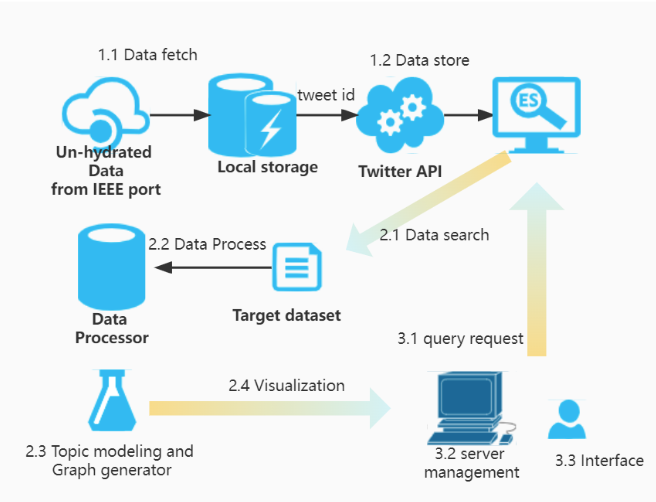
\includegraphics[width=0.5\textwidth]{imgs/framework/framework.png}
\caption{System structure}
\label{fig:System structure}
\end{figure}
In dataset processing step, after importing data into Elasticsearch server in
batches, we choose a research scope and we get the target dataset from
Elasticsearch. By doing spatial query and filtering task, the target dataset
can be visualized into a map. Furthermore, after processing the data by using
techniques such as the regex filtering, tokenization and tagging, and
removing stop words, it is possible to apply a topic clustering model to get topics.


\subsection{Tweet Data Collection and Processing}
\subsubsection{Tweet Data Collection process}
The dataset we used is CORONAVIRUS (COVID-19) GEO-TAGGED TWEETS DATASET form
IEEE DataPort. Due to the tweets spreading policy. We can't access the
completed tweets content directly.  Thus. We use a transfer program named
Twarc to batch fetch tweets in the dataset. Twarc is a python package
that used to export tweets automatically.  The main principle is that Twarc
will make use of the registration information from twitter developer platform
and get the permission from Twitter. Then Twitter can monitor the whole
process of getting tweets. This way is completely legal and doesn't violate
the privacy protocols set by Twitter. But it also cause some issues. If the
tweets account is banned or the permission has been changed, we can't access
the content anymore. Normally Twitter doesn't send any warning message but
change the content of tweets to a prompt message. So some filtering process
is necessary to ensure that the data set is not contaminated with irrelevant
information. 

We collect data from March 2020 to March 2022. These data comes form hundreds
of single CSV files, Since they are stored by date. So a batch process is
necessary to import from these files. After that we store all of these data
to Elasticsearch, in order to facilitate subsequent steps to call. After
delete all the irrelevant information or the missing information data. The
whole memory size up to 142Mi. The number of useful pieces of information
reaches 388,719. However, the geographical distribution of this tweets is
very uneven. So we try to select states with large sample sizes as research
subjects.

\subsubsection{Tweet Data structure}
The original data contains tweets ID and sentiment score calculated by
database publisher Figure~\ref{fig:Tweet dataset}. We use tweets ID to
request twitter API in batch and get completed information, including
content, UTC time, geographic location. All of these information are fully
imported into the server after splicing with sentiment score.  In this
process, we will transfer the longitude and latitude to the geometry, then we
can apply some spatial operator to handle them. Time format is another point
in this way, we transfer all the time appearing in our project to UTC format.
Then all filtering of time will be consistent. 
\begin{figure}[h]
\centering
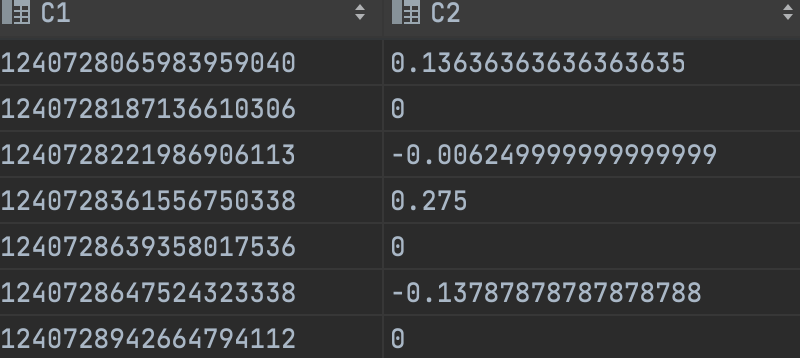
\includegraphics[width=0.5\textwidth]{imgs/row_tweets.png}
\caption{Tweet dataset structure}
\label{fig:Tweet dataset}
\end{figure}
\subsubsection{Tweet Data Pre-processing Method}
The pre-processing process includes regex filtering, tokenization and tagging,
removal of stop words (Figure~\ref{fig:Tokenization and tag}). Regex
filtering process used to delete some proper noun or URL. We can also delete
all the hashtag or the emojis. Normal phrase or locations can also be a
optional. Basically, we will set different filtering rules according to the
task goals and model requirements. 

Tokenization and tag are important to our project. We use nltk package to
process the sentence in the tweets and decompose the content into single
words. Then we can filter for parts of speech and get more reasonable
results. 
\begin{figure}[h]
\centering
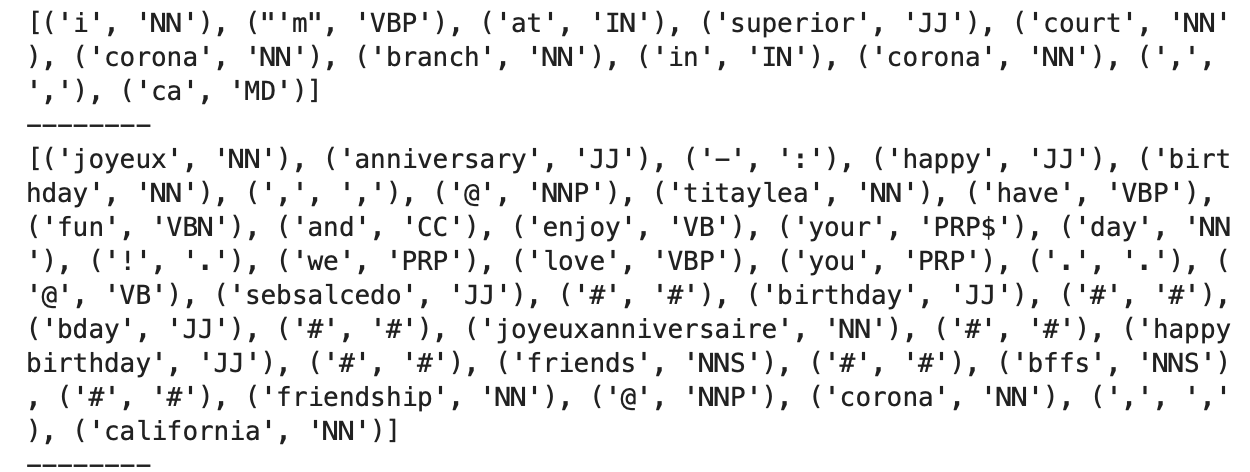
\includegraphics[width=0.5\textwidth]{imgs/tokenization.png}
\caption{Tokenization and tag}
\label{fig:Tokenization and tag}
\end{figure}
The purpose of removal of stopwords is to avoid distractions from common words
on the topic. The nltk package provide a library of stopwords and we can set
our own list of common words based on the theme. It's an important step to
get good performance of machine learning models and we can adjust it to fit
the current strategy we used. It's a part of fine turning. 

\subsection{Topic Clustering}
For topic clustering, first we collected the data from Elasticsearch server by
filtering using spatial queries. The data had text, geo-tag and tweet ID as
data columns. Since the text contained lots of unwanted strings or
characters, we needed to clean the data. 

Some tweet contains hypertext URL such as: 
\begin{verbatim}
    https://t.co/{tweet_id}
\end{verbatim} and some other URLs as shown in (Figure~\ref{fig:Right-most column}):
% \begin{figure}[H]
%     \centering
%     
\includegraphics[width=0.5\textwidth]{url.JPG}
%     \caption{An example of Tweet containing URL}
%     \label{fig:tw_url}
% \end{figure}
    
We needed to filter these unnecessary texts from the actual twitter data using
some regular expression operator and cleaning the part that corresponds to
those specific terms. We also needed to remove all the punctuation marks so
that it drops the redundant and recurring feature that don't contribute to
the clustering.

Example of these regular expression technique is shown in the (Figure~\ref
{fig:Shows the conceptual}): 
\begin{figure}[H]
    \centering
    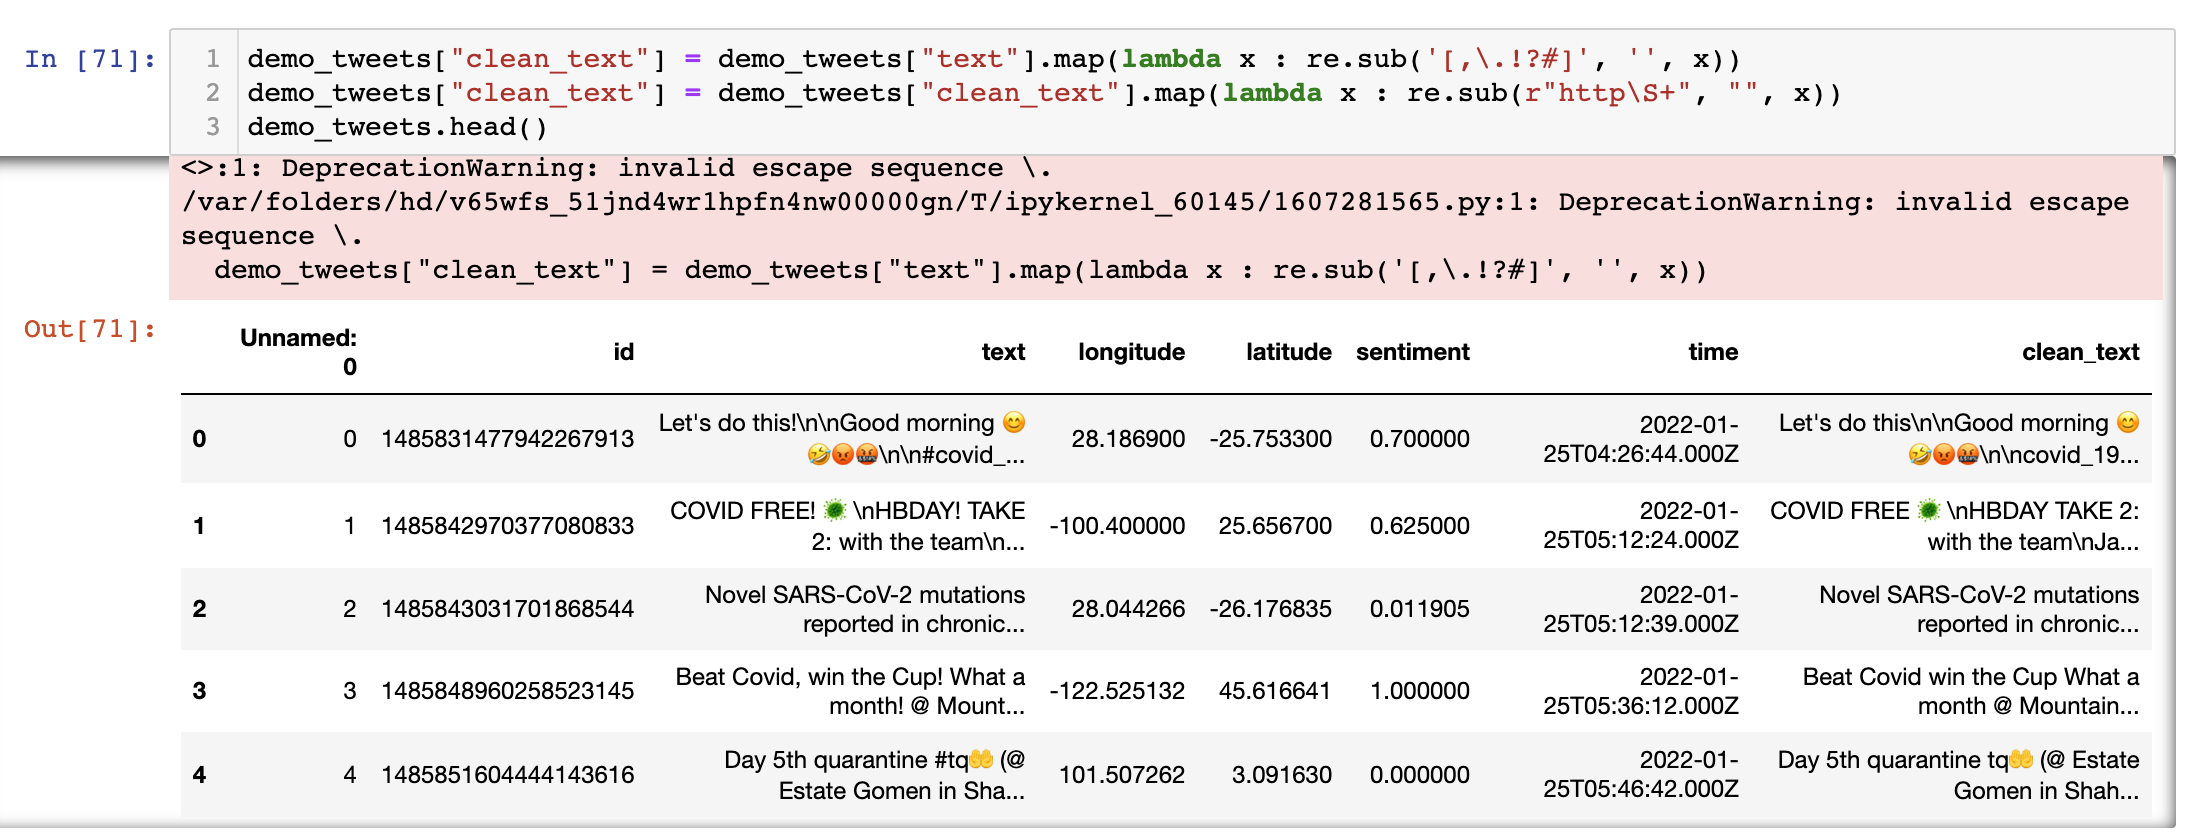
\includegraphics[width=0.5\textwidth]{imgs/cleaning_w_regex.png}
    \caption{Right-most column showing cleaned text with Regex}
    \label{fig:Right-most column}
\end{figure}



In the (Figure~\ref{fig:Completed dataset}), the circle size of the term
clusters visualize the frequency of the terms appearing in the documents.

\subsection{Spatial Data Mining and Visualization}
\subsubsection{Data Mining Method}
First, we import all data into Elasticsearch server. Then we get to use
different type of query instructions to request data on demands. In order to
narrow down the scope of our research range, we build two methods and
well-package them, which are query by time and query by location.
Regionally-targeted requests are often broken down by state. So we use two
key steps to accomplish the filtering to the data. First, get the minimum
circumscribed rectangle of the state to search. Next, filter out all points
outside  the boundary by spatial operations. 

\subsubsection{Visualization Method}
We use matplotlib to generate the map automatically. At the same time, we
distinguish different types of points and areas by marking the map with
different colors. Depending on the focus, we'll display a national map or a
state map.
\section{Experiments}
\label{sec:exp}
We apply our research method experimentally on a large spatial-temporal dataset collected from IEEE dataport. By compare the result with real events in Coronanet which records government responses to coronavirus, we evaluate the plausibility of the method. The result shows several points of interest in a specific time period and the details within each topic.
\subsection{Dataset Description and Experiment Setup}
Dataset: \\
The dataset we used is CORONAVIRUS (COVID-19) GEO-TAGGED TWEETS DATASET form IEEE DataPort. Due to the tweets spreading policy. We can’t access the completed tweets directly. Thus. We use a transfer program named Twarc to batch fetch every tweet in the dataset. Twarc is a python package that is used to export tweets automatically. The main principle is that Twarc will make use of the registration information from twitter developer platform and get the permission from Twitter. Then Twitter can monitor the whole process of getting tweets. This way is completely legal and doesn’t violate the privacy protocols set by Twitter. But it also causes some issues. If the tweets account is banned or the permission has been changed, we can’t access the content anymore. Normally Twitter doesn’t send any warning message but changes the content of tweets to a prompt message. So some filtering process is necessary to ensure that the data set is not contaminated with irrelevant information.


Metrics:\\
We use silhouette factor to evaluate the performance of clustering. For storyline generation, we based on rationality of the time series and topic keywords. 


Topic mining:\\
To evaluate the quality of generated topics, we focus on both the content of the topic itself and the distribution of the topic. 


In the experiment, each topic consists of a series of related sentence vectors. We use high-frequency words in WordCloud to show the content of the topic. Besides, We also output one of the most representative sentences in each topic as supporting evidence. 


The distribution of clusters in the vector space is another indicator of the quality of the results. The projection of vectors in two-dimensional space can intuitively see the distribution of the cluster. In order to verify the temporal relevance of the topic we also use the time label of the topic vector as the third axis to generate a three-dimensional vector distribution map.


Comparison Models: \\
We propose a combination of lda and bert methods to produce high-quality sentence vectors. To verify the advantages of this approach, we output the clustering results using bert and LDA separately. We make a comprehensive assessment based on the quality of the topics and timelines generated by each method
\subsection{Results and Discussion}
\subsubsection{Derivation of topic}
\begin{figure}[h]
\centering
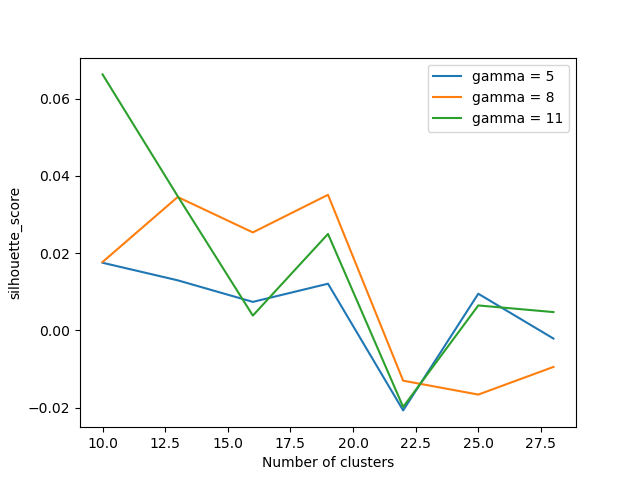
\includegraphics[width=0.5\textwidth]{imgs/2d_derivation.png}
\caption{2d derivation}
\label{fig:2d_derivation}
\end{figure}


\\In Fig~\ref{fig:2d_derivation}, we adjust the number of clusters and weight ratio of the vector structure to get the best silhouette score. The quality of the generated storyline will also be a reference. 
\subsubsection{Topic content}
\subsubsection{Evaluation of clustering}
\subsubsection{Storyline}
\subsubsection{Model comparision}


\section{Discussion}
In this project we propose a model mapping some spatio-temporal data into a
map once getting such dataset from Twitter. This model successfully take
pre-processed twitter data and return visualized result of distribution of
such data. With machine learning-based binary classification, the
spatio-temporal data now can have sentiment information as well, therefore it
is possible to visualize the the trend of people's opinion by regions and
time. This model has potential to be developed as an API automatically return
visualized map of distribution of sentiments on some issues. This may
contribute the government decision maker to refer to public opinion on a
specific issue they are interested in. 

Visualization of the spatial feature flow as the temporal data progresses is
an integral part of data warehousing and data mining techniques. Spatial data
mining requires specific trend recognition in order to make successful
conclusive argument which is visualized using the visualization technique. In
this project, we have used Geo Pandas to visualize our spatial data using
designated spatial operator. In our future studies, we would like to make the
model propose the trends in spatial data flow in maps which can be visualized
using the similar libraries.\\

\begin{figure}[H]
\centering
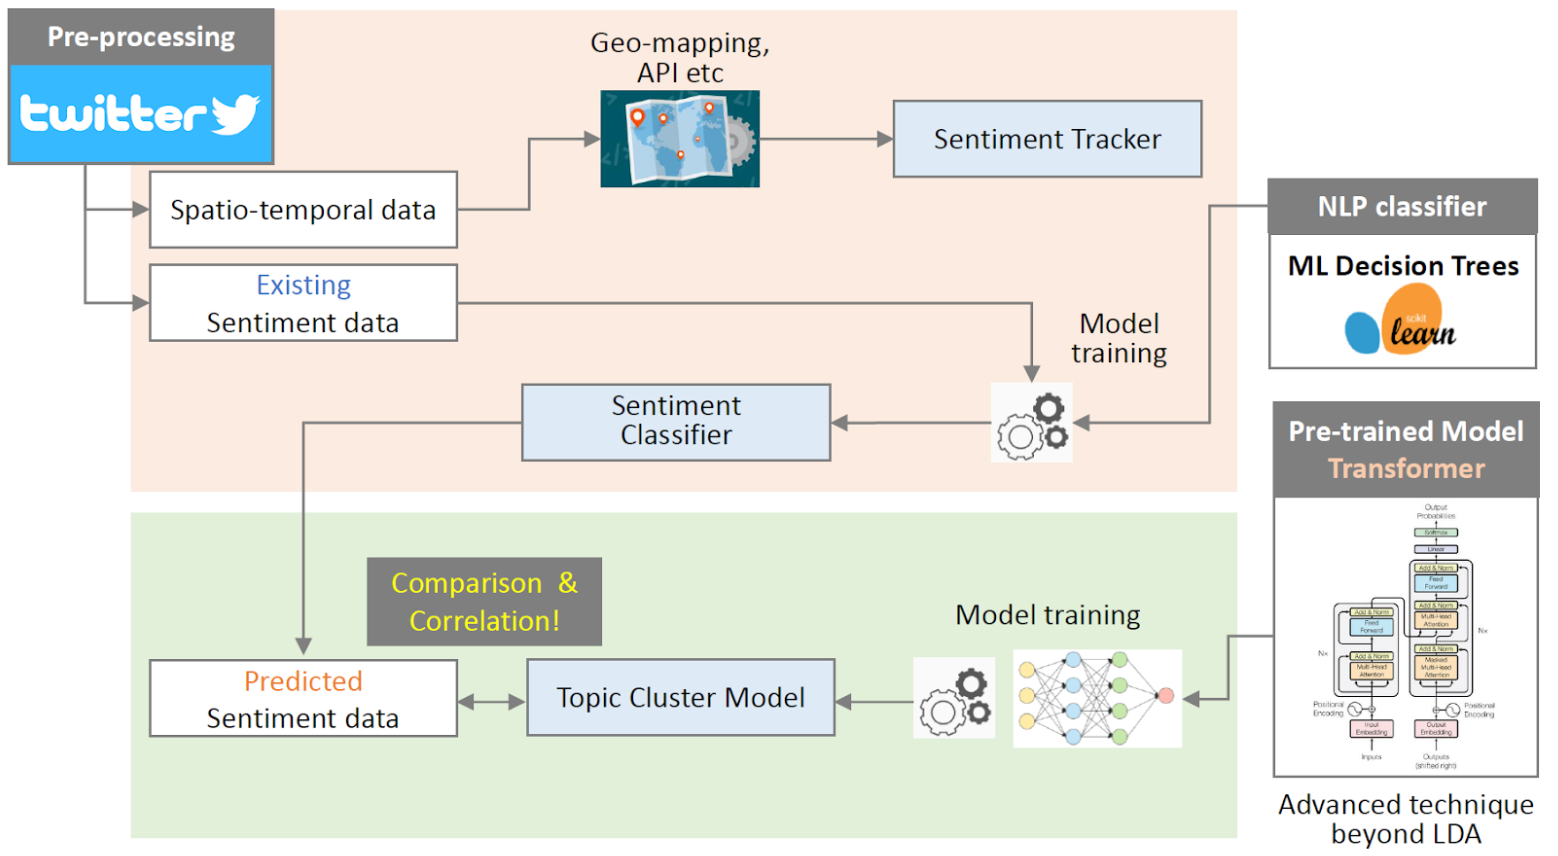
\includegraphics[width=0.5\textwidth]{imgs/Research_Process.png}
\caption{\label{fig:Research process}Future plan}
\end{figure}

However it still has a long way to go in that it is too simple for disclosing
some deeply meaningful implications. At present, since our model just
provides the spatio-temporal view of the public opinion about an issue, it
lacks further analysis about what specific topics are to be drawn from this.
To dig into this issue, we will do detailed topic clustering task to classify
how many different sub topics can be drawn from the overall topic of Covid-19
outbreak. Our topic for twitter dataset are filtered by the topic pandemic.
However this is too simple. Therefore in the longer run, we should proceed to
sub-topic clustering to get detailed areas under the single main topic. For
example, they might be either government's specific policy about the pandemic
or public opinion about some vaccine company's business guideline, and etc.

In this project, we have chosen a static method for topic clustering which is
Latent Dirichlet Allocation (LDA). Although this is static and an old method
compared to the modern deep learning approaches, our result shows its
relevancy in this domain is still present. The current research that are
going on, a lot of the authors are using LDA to get a primary insight in the
dataset that they compare with their model as a baseline. In the coming days,
our research will focus on the modern approaches using deep learning to make
compact and deployable topic clustering model.

One promising candidate for the model is the Transformer. This is a greatly
applied model architecture in Natural Language Processing now, which is based
on the core technology called the \textit{attention mechanism}. Our team
belive this should be an appropriate alternative current LDA to do the
detailed topic clustering task (Fig.21). 
[\section{Conclusion}
In this project, our team carried out a machine learning-based spatial
modeling of sentiment towards the pandemic. A rationale for this research
comes from the increased interest on analyzing a lot of issues related to
pandemic by using machine learning in academia. We have been pursued to
combine the ML and Deep Neural Network (DNN) with our spatial-data mining
technology so that this study contributes to the field by producing deeper
implications.

As a dataset for sentiment analysis the importance of Twitter dataset can not
be overstated. In recent days of DNN era, the public opinion expressed in
twitter became a valuable resource for numerous tasks including such
sentiment prediction. We paid attention on the applicability of DNN on the
Twitter dataset for the pandemic issue. By using some applications such as
Twarc and Elasticsearch we collected and stored such related dataset into our
own repository, and spatial datamining task such as querying is followed. By
doing such spatial query and filtering task, the target dataset could be
visualized into a map. Furthermore, we develop a sentiment classifier by
adopting the decision tree in Machine Learning. This module analyzes people's
opinion in tweeter data and classifies it into positive or negative, by
getting trained with pre-built sentiment score.

However, there are still another important task remained to achieve our team's
final goal. Since our current model simply mine the spatio-temporal dataset
and show how people's opinion is distributed differently by regions and time,
it requires to do further research to draw deeper implications for
contributing academia. Therefore, we plan to build a sub-topic clustering
module using Transformer and compare its result with our predicted sentiment
score. With adopting such a new NLP model architecture, it is expected to
track a distribution of public opinion on detailed issues, e.g., government
policy on social distancing, vaccine supply, etc., so that the study can have
practical implication to decision makers. 

\bibliographystyle{IEEEtran}
\bibliography{references}

\end{document}